% intro.tex aus dem Projekt PdU
% ADAPTIERT FÜR DAS PROJEKT RW am 2.7.2015
\RWch{Vorwort}\hbox{}\par\noindent\markboth{\kopfzeilenfmt{Vorwort}}{\kopfzeilenfmt{Christian Tapp}}%
\rule{0pt}{1.4\baselineskip}Seit ihrem Erscheinen im Jahre 1834 hat Bolzanos \werk{Religionswissenschaft} keine erschwingliche Ausgabe mehr erlebt. Dies ist für die Philosophie, vor allem für die Religionsphilosophie, umso bedauerlicher, als Bolzano zu Recht als \anf{Großvater der Analytischen Philosophie} (Dummett) gilt -- und wann, wenn nicht heute ist deren Zeit? Hier also ist die Ausgabe!\\[\baselineskip]
Zu danken ist v.\,a.\ den studentischen Hilfskräften Fr. Daniel Tibi OSB, Magdalena Ruschkowski, Franziska Pircher und Sr.~Klara (Katja) Hölzl, die mit viel Sorgfalt und Mühe den Rohtext erstellt und bei den verschiedensten Recherche- und Korrekturschritten tatkräftig mitgearbeitet haben.\\[\baselineskip]
Bochum, an einem künftigen Tag des Jahres 2020\\[\baselineskip]
\hbox{}\hfill\textit{Christian Tapp}

\RWch*{\hbox{}}\vspace{-0.35\baselineskip}
%\makeatletter\clearpage\pagestyle{normal}\@makeschapterhead{\hbox{}}\setcounter{pdusecnum}{1}\par\noindent\vspace{-0.35\baselineskip}%
%\zit{
\anf{Doch den entschiedensten Vertheidiger hat das Eigentlich-Un"-end"-li"-che \auslass\ in einem höchst scharfsinnigen Philosophen und Mathematiker unseres Jahrhunderts, in Bernhard [!] Bolzano gefunden, der seine betreffenden Ansichten namentlich in der schönen und gehaltreichen Schrift: \einfanf{Paradoxien des Unendlichen, Leipzig 1851} entwickelt hat, deren Zweck es ist, nachzuweisen, wie die von Skeptikern und Peripathetikern aller Zeiten im Unendlichen gesuchten Widersprüche gar nicht vorhanden sind, sobald man sich nur die freilich nicht immer ganz leichte Mühe nimmt, die Unendlichkeitsbegriffe allen Ernstes ihrem wahren Inhalte nach in sich aufzunehmen.}\\[0.5\baselineskip]
\textsc{Georg Cantor}, \textit{Grundlagen einer allgemeinen Mannichfaltigkeitslehre}, Leipzig: Teubner 1883 = Ueber unendliche, lineare Punktmannichfaltigkeiten, 5., in: Mathematische Annalen 21 (1883), S.\,545--591, hier 560.%}

\RWch{Einleitung}\markboth{\kopfzeilenfmt{Einleitung}}{\kopfzeilenfmt{Christian Tapp}}
\vspace{-1.5\baselineskip}
\PdUsec{Der Autor}
\parpic[r]{\setlength{\fboxsep}{0pt}\setlength{\fboxrule}{0.25pt}\framebox{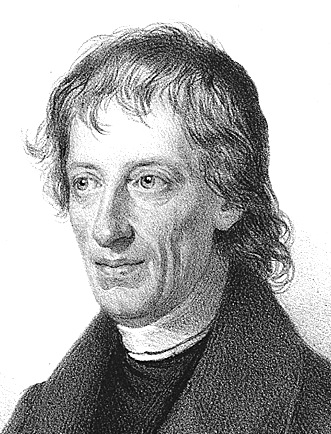
\includegraphics[scale=0.32]{bolzano-abb/portrait.jpg}}}
\noindent Bernard Bolzano war in vielerlei Hinsicht ein außergewöhnlicher Mensch. Als Wissenschaftler verband er so verschiedene Begabungen wie die eines Mathematikers, eines Philosophen, ein"-es Logikers und eines Theologen. Er war katholischer Priester und ein seine Zuhörer begeisternder Hochschullehrer. Er war ein tiefgläubiger Mensch und fühlte sich ganz der Vernunft verpflichtet.  Gedankliche Klarheit, begriffliche Präzision und argumentative Untermauerung seiner Standpunkte galten ihm \anf{als Grundlage für ein vernünftiges, gottgefälliges Leben zum Wohl der Allgemeinheit}.\footnoteA{%
	\lit[11]{Strasser2001}.}
Bolzano ist, dem Philosophen Michael Dummett zufolge, Urgroßvater der analytischen Philosophie.\footnoteA{%
	\lit[167]{Dummett1988}.}
Von ihm stammt der Satz von Bolzano-Weierstraß, den jeder Mathematikstudent heute in seinem ersten Semester 
lernt.\par

\PdUsec{Der Text}
Von der \RWbet{Religionswissenschaft} gibt es fünf Versionen, nämlich 
\begin{compactenum}[1.]
\item[1.] Bolzanos schriftliche Fassung seines ersten Vorlesungszyklus zum Thema;
\end{compactenum}
dann drei Fassungen, die zu Bolzanos Lebzeiten erarbeitet wurden und seine Zustimmung fanden:
\begin{compactenum}[1.]
\item[A] Die 1834 publizierte Fassung,
\item[A$_1$] Bolzanos Überarbeitung von A in seinem Handexemplar sowie
\item[B] Eine im Jahre 1818 erstellte Abschrift seiner Manuskripte für die Studienhofkommission
\end{compactenum}
und schließlich
\begin{compactenum}[1.]
\item[5.] der Text in der Bernard-Bolzano Gesamtausgabe [=GA], Reihe 1, Bände 6/1--2, 7/1--2 und 8/1--4.
\end{compactenum}
Bolzano las seit 1805 regelmäßig einen viersemestrigen Zyklus zur Religionslehre. Der Text des ersten Zyklus ist 1. In den folgenden Jahren überarbeitete Bolzano sein Manuskript stetig. Als er 1818 der Studienhofkommission in Wien seine Arbeiten vorlegen musste, legte er B vor, einen Text, der von einem professionellen Schreiber verfasst, von Bolzano jedoch detailliert korrigiert und im Einzelnen approbiert wurde. 1834 schließlich publizierten Schüler Bolzanos das \RWbet{Lehrbuch der Religionswissenschaft}  (= A) anonym bei Seidel im bayrischen Sulzbach, denn  Bolzano durfte seit seiner Entlassung 1819 im Habsburgerreich nicht mehr publizieren. Bolzano zeigte sich mit dem durch seine Schüler eigenständig redigierten Text relativ einverstanden, wollte aber für eine zweite Auflage Umarbeitungen vornehmen. Zu diesem Zweck ließ er sich ein Exemplar des ersten Bandes vom Buchbinder mit leeren Seiten durchschießen, auf die er seine Überarbeitungen eintrug -- so entstand der Text A$_1$. Der Text der Gesamtausgabe folgt im Wesentlichen A$_1$, gibt aber auch Varianten aus $B$ an.\par
% UNZUVERLASSIGKEIT VON GA
Ein Problem mit der ansonsten äußerst verdienstvollen kritischen Edition der Gesamtausgabe ist jedoch, dass sie häufig nicht zuverlässig ist:
Sinnentstellende Verschreibungen (\zB\ \anf{Richtigkeit} statt korrekt \anf{Nichtigkeit} in RW I 10 oder RW IIIa 18); fehlende gewichtende Zusätze (\zB\ \anf{eine höhere Denkfähigkeit} statt korrekt \anf{eine bedeutend höhere Denkfähigkeit} in RW I 13). Nicht-berücksichtigte Korrekturen von Bolzanos Hand, die Sinnstörungen vermeiden (\zB\ \anf{für Laien bestimmt} (wie in \Alabel ) statt \anf{für Nicht-Theologen bestimmt} in RW I 24).
Daher folgt diese Studienausgabe im Wesentlichen dem Text \Alabel\ der gedruckten Ausgabe von 1834. Nach Möglichkeit werden Bolzanos eigene Verbesserungsvorschläge aus der A$_1$ übernommen. 
Diese Studienausgabe folgt im Wesentlichen dem Text der Gesamtausgabe, d.\,h. der Vorlage \A1label\ bzw. \Alabel , und zwar vor allem aus pragmatischen Gründen. So ist dieser Text relativ gut digitalisierbar. Eine eigene Edition von B machte eine Menge zusätzlichen Aufwands nötig und gehörte wohl eher in die Reihe der unveröffentlichten Schriften in der 
Gesamtausgabe.\par
Grundsätzlich wird aber in Folgendem von der GA abgewichen:
\begin{aufza}
\item Grundsätzlich wird zugunsten des Textumfangs dieser Studienausgabe nur derjenige Text der GA zugrundegelegt, der auch in \Alabel\ bzw. \A1label\ vorkommt. Zusätzliches Material wie die frühere Fassung der Vorrede, das \anf{Vorwort} (GA I 6/1, S. 19--22), oder die vielfältigen Auszüge von Varianten aus B in den Anhängen der Bände der GA werden weggelassen.
\item In \Alabel\ waren nahezu alle Textabsätze durchnummeriert. Die GA löscht diese Nummerierungen (vermutlich, weil Bolzano selbst sie in A$_1$ gelöscht hat) und setzt die Unternummerierungen dafür eine Ebene höher (\dh\ eine nachgeordnete Aufzählung beginnt nun mit arabisch 1., während sie in A mit lateinisch a. begann -- dafür nummeriert arabisch 1. eben den Absatz). Diese Änderung gegenüber A wird jedoch in GA weder verzeichnet noch beschrieben. Sie wird auch nicht durchgehalten, sodass sich ein uneinheitliches Bild ergibt: In GA I 6/1--2 die gegenüber A geänderte Nummerierung, in GA I 7 \& 8 die ursprüngliche Nummerierung aus A. Hier wird die ursprüngliche Nummerierung aus A einheitlich und durchgängig verwendet.
\end{aufza}
Für die konkrete Textgestalt wurden Bolzanos eigene Wünsche, soweit sie aus seinen handschriftlichen Überarbeitungen und Hinweisen in A$_1$ ersichtlich sind, nach Möglichkeit berücksichtigt: 
\zit[{Bolzano in A$_1$, S. 1 am Rande; zit. n. GA I 6/1, S. 41}]{%
Sollte es nicht besser seyn, \auslass\ wenn die §§ Nummern durch das ganze Buch eben neben der Seitenzahl auf jedem Blatte angezeigt würden, wodurch das Nachschlagen erleichtert würde?
}
Am Beginn des Inhaltsverzeichnisses verlangte Bolzano am Ende der Überschriften der Paragraphen 11, 13 und 14, insofern es sich bei diesen und unter den ersten 14 Paragraphen auch nur bei diesen um vollständige Sätze handelte, einen Punkt. Ab Paragraph 15 hingegen hat er das nicht mehr korrigiert, obwohl etwa die Paragraphen 15--18 alle ganze Sätze als Überschriften tragen. Vermutlich hat er diese Korrekturmaxime also wieder aufgegeben. Mithin werden die drei genannten Punkte nicht übernommen.\par
Wenn Bolzano durch inkonsistente Korrekturen die Möglichkeit zur Vereinheitlichung oder sonstiger Verbesserung des Textes gibt, wird sie vorgenommen. So korrigiert er im Inhaltsverzeichnis nicht, dass bei § 23 von \erganf{Offenbarung}, in der ganz parallel gestalteten Überschrift von § 24 jedoch von \erganf{Offenbaren} die Rede ist. In den betreffenden Kapitelüberschriften heißt es später jedoch beide Male \erganf{Offenbaren}, sodass wir dies auch im Inhaltsverzeichnis vereinheitlichen.\par
Wenn aus Bolzanos ausführlicher Korrektur des 1.~Bandes eine klare Intention bzgl. der Schreibungen hervorgeht, wird diese Intention auch in den anderen Bänden umgesetzt. So hat er bspw. aus dem Wort \anf{Willkühr} und Ableitungen wie \anf{unwillkührlich} im 1.~Band konsequent (wenn auch nicht überall, \zB\ nicht im letzten Satz von \RWparnr{137}) das h gestrichen. 

Weitere Hinweise zur Gestaltung dieser Edition:
\begin{aufza}
\item Grundsätzlich bleibt die Orthographie so wie zu Bolzanos Zeit. Dies schränkt die Lesbarkeit kaum ein und vermittelt dem Leser dafür etwas von dem authentischen \anf{Flair} des 19.~Jahrhunderts, wenn er beispielsweise \anf{Princip}, \anf{nöthig} oder \anf{Gesammtglaube} liest. 
\item Bolzano hat Zitate von Texten in der Regel nicht in Anführungszeichen eingeschlossen. (In A werden kaum Anführungszeichen verwendet. Bolzano scheint sie auch nicht in A$_1$ nachgetragen zu haben.) Um die Lesbarkeit und die Identifikation von Zitaten zur erleichtern, werden in dieser Ausgabe Zitate oder zitatnahe Paraphrasen fremder Texte nach Möglichkeit in Anführungszeichen eingeschlossen. Dabei werden deutsche Anführungszeichen (\eanf{\ }) dort verwendet, wo Bolzano selbst Anführungszeichen gesetzt hat. Wir ergänzen hingegen inverse französische Anführungszeichen (\erganf{\ }) als Markierung von Zitaten, etwa wenn im Apparat Literatur nachgewiesen wird. Allerdings muss man stets im Kopf behalten, dass Bolzano häufig eher paraphrasiert als wörtlich zitiert. Dennoch erhöhen diese Zeichen die Lesbarkeit, insofern man schnell sieht, wo das Referat (sei es wörtlich oder paraphrasierend) beginnt und endet. Keine Anführungszeichen werden hingegen dort ergänzt, wo nach heutiger Konvention ein Wort erwähnt und nicht gebraucht wird, und auch dort nicht, wo man wörtliche Rede heute meist in Anführungszeichen setzen würde. Referiert Bolzano beispielsweise eine Passage aus einem sokratischen Dialog, so wird diese Passage als Ganze in Anführungszeichen gesetzt, die einzelnen Redebeiträge der Dialogteilnehmer hingegen nicht. Ebenso wird verfahren bei Jesus-Worten: Sind es biblische Zitate (oder Paraphrasen), so werden die Anführungszeichen \erganf{\ } ergänzt, als wörtliche Rede einer Person hingegen werden keine Anführungszeichen hinzugefügt.
% \erganf verwenden für ergänzte Anführungszeichen, d.h. solche, die nicht in A vorkommen
\item Die Zeichensetzung folgte im 19.~Jahrhundert anderen Üblichkeiten als heute. Bolzano setzt Kommata regelmäßig an Stellen, an denen nach heutigen Regeln keine gesetzt werden, etwa vor \anf{und} und \anf{oder} in Beiordnungen von Sätzen, die ein gemeinsames Subjekt haben, zwischen \anf{sowohl} und \anf{als auch} sowie vor Vergleichen mit \anf{als}. Grundsätzlich bestanden mehr Freiheiten. So setzt Bolzano Kommata auch als rhetorische Untergliederungen ein. Die Zeichensetzung in dieser Ausgabe folgt im Wesentlichen Bolzanos eigener Zeichensetzung in Ausgabe A. Abgewichen wird davon nur, wenn es naheliegt, dass nach Bolzanos mutmaßlichen eigenen Zeichensetzungsprinzipien ein Fehler vorliegt -- wie etwa dann, wenn bei einer Folge offensichtlich beigeordneter Sätze ohne erkennbaren Grund nur einmal ein Semikolon anstelle eines Kommas steht, ein Punkt sowohl vor als auch nach einem eingeklammerten Ausdruck am Satzende steht oder wenn ein Komma am Satzende auftaucht und der Beginn des nächsten Satzes großgeschrieben wird usw. -- oder sich zumindest eine andere Zeichensetzung nach Bolzanos eigener Systematik nahelegt -- wie etwa dann, wenn er eine Reihe von Bibelstellen nach dem Schema \anf{Stellenangabe - Doppelpunkt - Paraphrase} angibt und der Doppelpunkt in Einzelfällen fehlt.
\item Bolzanos spezifische Form, Bibelstellen anzugeben, wird grundsätzlich beibehalten. So setzt er zwischen Kapitel- und Verszahl ein Komma ohne Leerzeichen und schließt die Stellenangabe mit einem Punkt ab, der für heutige Lesegewohnheiten ungewöhnlich ist, aber im Sinne einer Ordnungszahl durchaus Sinn macht: \anf{11,7.} hat er wohl gelesen im Sinne von \anf{Kapitel 11, \RWbet{siebter} Vers}. Ebenfalls zugunsten der besseren Lesbarkeit wird zwischen aufgezählten Bibelstellenangaben ein Satzzeichen eingefügt. Wir schreiben also \anf{1\,Mos.~1,26.; 3,22.; 11,7.} statt \anf{1\,Mos. 1,26. 3,22. 11,7.}
\item Die Orthographie wird weitgehend so belassen, wie Bolzano sie mutmaßlich anwandte. Mithin werden im 19.~Jahrhundert übliche Schreibungen wie \anf{Thal}, \anf{Gesammtheit}, \anf{insgesammt} u.ä. beibehalten. Nur offenkundige grammatikalische oder orthographische Fehler werden berichtigt wie z.B. \anf{Aeußerungen über Gottes dreifache Persönlichkeit} anstatt \anf{\auslass\ dreifacher \auslass}, oder etwa \anf{\RWgriech{basile'ian Jeo~u o>u klhronom'hsousin}} statt \anf{\RWgriech{\auslass\ klhronom'hsousi}} (in RW IIIb 143 ausdrücklich aus der Bibelstelle \RWbibel{1\,Kor}{1\,Kor}{6}{9} zitiert). In relativ eindeutigen Fällen wie diesen, werden die Änderungen  stillschweigend vorgenommen.  Änderungen gegenüber A, bei denen nicht sicher ausgeschlossen werden kann, dass die fehlerhaft scheinende Schreibung irgendeinen Sinn haben könnte, werden im Apparat vermerkt.
\item Nach heutigen Regeln werden am Ende von Überschriften keine Punkte gesetzt. Daher werden die Punkte nach den Überschriften der Paragraphen weggelassen. Da die Überschriften der Hauptteile und anderen größeren Abschnitte jedoch in aller Regel mehrere Teile haben, die eh durch Punkte abzutrennen sind, werden hier zur Vereinheitlichung auch die Endpunkte beibehalten.
\item Einige Besonderheiten ergeben sich aus Bolzanos teilweiser Überarbeitung von \Alabel\ zu \A1label . In \Alabel\ werden Adjektive, die zwischen \anf{alle} und einem Substantiv stehen, wie heute üblich schwach flektiert (\anf{alle christlichen Weltweisen}); gelegentlich hat Bolzano dies in \A1label\ jedoch ausdrücklich zur starken Flexion hin korrigiert (\anf{alle christliche Weltweisen}). Da die starke Flexion nach \anf{alle} heute vollkommen unüblich geworden ist und da Bolzano diese Korrekturen selbst in dem Teil der RW, den er intensiv überarbeitet hat, nicht immer durchführt, weichen wir hier zugunsten der besseren Lesbarkeit von seinem Willen ab und verwenden die schwache Flexion.
\item Sowohl in der Druckfassung \Alabel\  als auch in Bolzanos Überarbeitung \A1label\ wird gelegentlich \anf{allmählich} und gelegentlich \anf{allmählig} geschrieben. Da die Orthographie heute nur noch \anf{allmählich} kennt, wird dahingehend vereinheitlicht. Anders hingegen bei Variationen, bei denen auch heute noch beide Formen als korrekt gelten. So werden Bolzanos Wechsel zwischen \anf{-es} und \anf{-s} bei den Genitiv-Endungen nicht vereinheitlicht (\anf{des Christenthums} und \anf{des Christenthumes}). Dasselbe gilt für den gelegentlichen Ausfall des \anf{e} bei Worten wie \anf{anderen} / \anf{andren}. 
\item Die Informationen über Varianten von \Blabel\ im Verhältnis zu \Alabel\ wurden der \GAlabel\ entnommen. 
\item Auf Nummern von Absätzen oder Ähnlichem wurde in \Alabel\ durchgängig mittels \anf{Nr.} Bezug genommen. Bolzano hat dies in den Teilen, die er überarbeitet hat, konsequent zu einer Graphie geändert, die offenbar für das Lateinische \anf{numero} oder das Französische \anf{numéro} steht: ein \anf{n} mit einem hochgestellten \anf{o} und einem darunterstehenden Punkt. Diese Schreibweise ließ sich nicht eindeutig einer der im europäischen Sprachraum üblichen Varianten wie No, No., N$^{\mathrm{o}}$, n$^{\mathrm{o}}$, n$^{\mathrm{o}}\!.$, n$^{\underline{\mathrm{o}}}$ oder Ähnlichen zuordnen. Daher wurde mit \no\ eine Drucktype entworfen, die seiner eigenen Schreibung möglichst nahekommt.
\item Wenn eine Nummerierung hinzugefügt worden ist, die in \Alabel\ nicht vorkommt, wird dies angemerkt.
\item Einfache Ergänzungen ggü. den Vorlagen werden in eckige Klammern gesetzt ([\auslass ]), bspw. wenn Bolzano RW I 25 eine Fußnote hinzufügt, die mit \anf{gestorben den \auslass} endet, wird das Todesdatum des Betreffenden in eckigen Klammern hinzufügt: \anf{gestorben den [11.\,Oktober 1834]}. Wird hingegen ein ganzes Wort ausgelassen, wird dies in den Anmerkungen vermerkt.
\end{aufza}

\endinput